\section{Обзор существующих решений}
\label{sec:Chapter2} \index{Chapter2}

% Здесь надо рассмотреть все существующие решения поставленной задачи, но не
% просто пересказать, в чем там дело, а оценить степень их соответствия тем
% ограничениям, которые были сформулированы в постановке задачи.

В современных компиляторах по типу GCC или LLVM (Low Level Virtual Machine) представлены несколько методов векторизации, которые направлены на оптимизацию выполнения программ за счет использования SIMD (Single Instruction, Multiple Data) инструкций. Поскольку принципиального различия в логике работы векторизаторов LLVM, GCC или других компиляторов нет, то обзор существующих решений можно провести на примере GCC.

\subsection{Циклическая векторизация}

\textbf{Циклическая векторизация} (Loop Vectorization) в GCC — это процесс преобразования циклов в код, использующий SIMD инструкции, для выполнения нескольких итераций цикла одновременно. Это позволяет значительно улучшить производительность за счет параллельного выполнения операций. Пример циклической векторизации представлен на рисунке ~\ref{cyclevec}.

\begin{figure}[!htb]
    \centering
    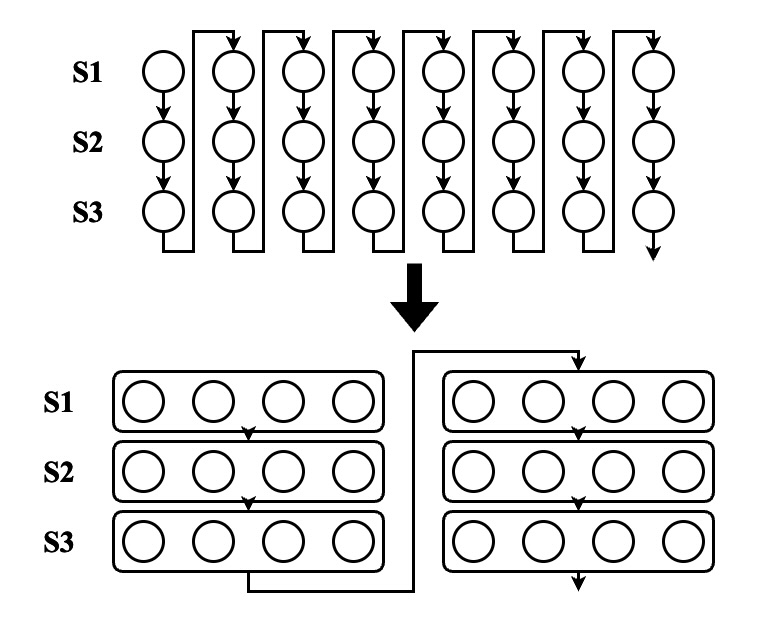
\includegraphics[scale=0.5]{cyclevec.jpeg}\\
    \caption{Циклическая векторизация в GCC}
    \label{cyclevec}
\end{figure}

Классический подход к векторизации базируется на теории анализа зависимостей данных. Первый шаг в этом анализе заключается в построении \textit{графа зависимости данных} (Data Dependence Graph, DDG). Анализ начинается с нахождения \textit{сильно связных компонент} (Strongly Connected Components, SCCs) \cite{liang2017vectorization}. Сильно связные компоненты ориентированного графа представляют собой его максимальные по включению сильно связные подграфы. Ориентированный граф называется \textit{сильно связным}, если любые две его вершины сильно связаны, то есть существует ориентированный путь от первой вершины ко второй и обратно.

SCC, состоящие из одного узла, представляют собой операторы, которые могут выполняться параллельно на данном уровне цикла. SCC, состоящие из нескольких узлов, обозначают операторы, участвующие в цикле зависимости, что может препятствовать векторизации цикла, если цикл не может быть разорван. Различают три типа зависимостей данных:

\begin{itemize}
    \item Запись после записи (Write after Write)
    \item Чтение после записи (Read after Write)
    \item Запись после чтения (Write after Read)
\end{itemize}

Пример всех трех зависимостей представлен на рисунке ниже:

\begin{figure}[!htb]
    \centering
    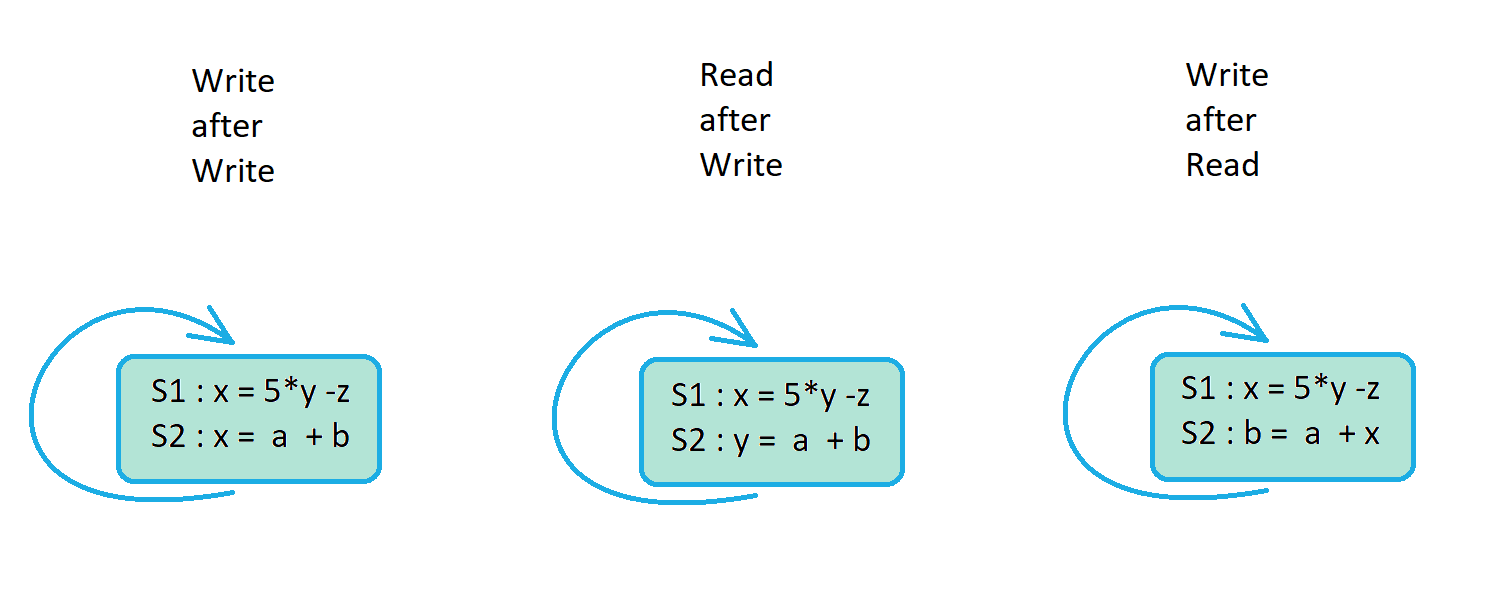
\includegraphics[scale=0.4]{dep.png}
    \caption{Пример зависимостей по данным}
\end{figure}

Помимо этого необходимо отсутствие сложного потока управления и невекторизуемых типов данных. Если условия векторизации выполнены, компилятор преобразует последовательные операции в векторные инструкции. Например, вместо выполнения сложения для каждого элемента массива последовательно, компилятор может создать векторную операцию, которая выполняет сложение нескольких элементов одновременно.

\subsection{SLP векторизация}
% расписать и применить цитирование
\textbf{SLP (Superword Level Parallelism)} – это метод векторизации, который фокусируется на объединении отдельных операций, выполняющихся над независимыми данными, в векторные операции. Этот метод необходим для векторизации последовательностей независимых инструкций в линейном коде, которые могут быть выполнены параллельно.

Существующий в GCC алгоритм может обрабатывать линейные участки кода в любом месте программы и, хотя он не ориентирован на циклы, SLP может векторизовать и код внутри циклов, где циклическая векторизация дает сбой. Для применения SLP векторизации в том или ином месте должен быть выполнен ряд условий, главными из которых также являются независимость операций по данным и отсутствие сложного потока управления \cite{chen2022all}. Тем не менее, авторы в работе \cite{shin2005superword} рассматривают способы SLP векторизации больших базовых блоков, содержащих некоторые конструкции ветвления. В качестве примера, подходящего для SLP, можно привести следующую функцию (рис. ~\ref{fooslp}), которая выполняет очень похожие операции со своими входными данными (a1, b1) и (a2, b2). Линейный векторизатор может объединить их в векторные операции.

\begin{figure}[!htb]
    \centering
    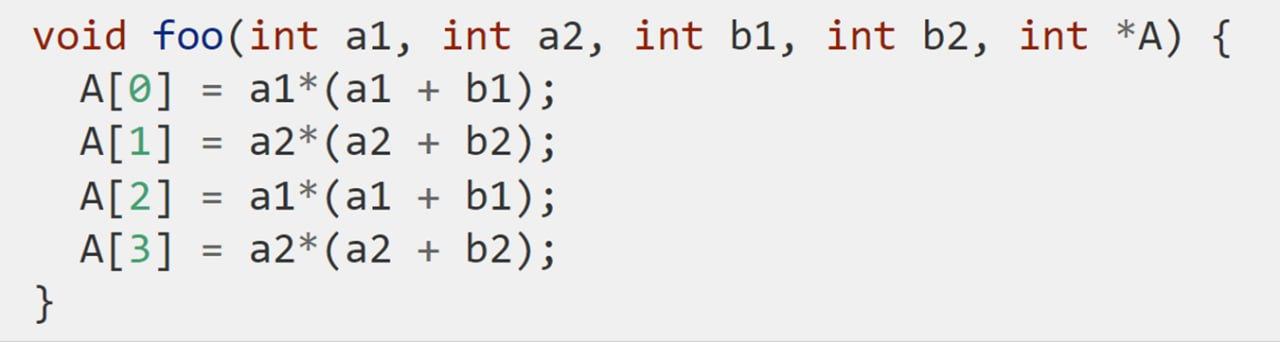
\includegraphics[scale=0.6]{fooslp.png}
    \caption{Пример ситуации, подходящей для линейной векторизации}
    \label{fooslp}
\end{figure}

\subsection{Векторизация потока управления}
В работе \textit{Control Flow Vectorization for ARM NEON} \cite{pohl2018control} были рассмотрены некоторые алгоритмы векторизации потока управления, а также был предложен способ векторизации операций загрузок из памяти на основе знания о страничной организации памяти для архитектур, которые не поддерживают \textit{маскированные} \cite{intel2017architecture} операции чтения и записи. Авторы работы, утверждают, что если на архитектуре выполнены следующие свойства,

\begin{itemize}
    \item аллоцированная память является непрерывной, т.е. массив хранится в непрерывной области памяти без пробелов и дырок
    \item доступ к памяти может быть выражен в виде линейного аффинного выражения, т.е. адреса строго возрастают или убывают
\end{itemize}

то код, содержащий операции ветвления, можно безопасно векторизовать, если во время исполнения будет происходить проверка на то, что элементы массива лежат и доступны в памяти. Авторы работы утверждают, что для этого достаточно проверить, что первый и последний элемент массива $cond[i]$, который состоит из 0 и 1, в условии ненулевые, что по сути является проверкой на то, что элементы массива доступны в пределах одной страницы памяти. На рисунке ~\ref{pohl1} представлен пример трансформации кода, позволяющий векторизовать блок кода, содержащий ветвление.

\begin{figure}[!htb]
    \centering
    \includesvg[scale=0.8]{pohl1.svg}
    \caption{Пример трансформации кода из статьи, добавляющей проверку во время исполнения и версионирование}
    \label{pohl1}
\end{figure}

Стоит обратить внимание, что здесь авторы используют идею \textit{маскированных} загрузок из памяти, где в качестве маски выступает массив $cond[i]$, содержащийся в условии, который по сути содержит информацию о том, какие значения векторизуемого массива будут использованы. Рисунок ~\ref{pohl2} показывает пример условной операции чтения из памяти, где условное выражение используется для \textit{маскирования} доступа в память.

\begin{figure}[!htb]
    \centering
    \includesvg[scale=0.5]{pohl2.svg}
    \caption{Пример использования условия в качестве \textit{маскирования} из статьи}
    \label{pohl2}
\end{figure}

\subsection{Остальные методы векторизации}
Для того, чтобы предоставить GCC свободу в выборе и применении векторизации, существует автовекторизация \cite{naishlos2004autovectorization}, которая позволяет компилятору самому выполнить векторизацию тех циклов, которые выгодно векторизовать и применить SLP там, где это необходимо. 

Помимо всего этого, пользователю доступен некоторый функционал для \textit{ручной векторизации}. GCC поддерживает использование встроенных функций (intrinsics) для конкретных SIMD наборов инструкций, таких как SSE, AVX и других. Программист может явно использовать эти функции для управления векторизацией.

В GCC присутствуют директивы $\#pragma$, которые могут быть использованы для указания компилятору векторизовать определенные участки кода. Например, $\#pragma$ $GCC$ $ivdep$ указывает компилятору игнорировать некоторые зависимости и векторизовать цикл. Также GCC поддерживает OpenMP. OpenMP (Open Multi-Processing) — это API, который позволяет реализовать многопоточность в программах на C, C++ и Fortran, предоставляя набор директив, функций и переменных среды для управления потоками.


\subsection{Проблема существующих решений}
Выше обсуждалось, что для применения векторизации в том или ином месте необходимо удовлетворить некоторому набору условий, одним из которых является \textit{сложный поток управления}. Сложным потоком управления можно считать последовательность выполнения операций или инструкций в программе, когда эта последовательность имеет множество ветвлений, циклов, вызовов подпрограмм и параллельных процессов. Такой поток управления может быть сложен для понимания и анализа, потому что в нем часто присутствуют следующие элементы:

\begin{itemize}
    \item \textit{Условные операторы}: Ветвления, такие как if, else, switch, которые приводят к выполнению различных блоков кода в зависимости от условий.
    \item \textit{Циклы}: Конструкции, такие как for, while, do-while, которые повторяют выполнение блока кода до тех пор, пока выполняется определенное условие.
    \item \textit{Рекурсия}: Функции, которые вызывают сами себя, что может усложнить анализ последовательности выполнения кода.
    \item \textit{Обработчики исключений}: Конструкции, такие как try, catch, которые управляют обработкой ошибок и исключений.
    \item \textit{Асинхронность и параллелизм}: Конструкции для работы с многопоточностью и асинхронным выполнением.
    \item \textit{Вложенные функции и лямбда-выражения}: Использование функций, определяемых внутри других функций, и анонимных функций.
\end{itemize}

Ленивые вычисления, обсуждаемые в главе 1.2.5, являются частным случаем сложного потока управления. Различные современные векторизаторы не способны объединять такие операции. Хоть авторы в работе \cite{pohl2018control} сильно продвинулись в этом направлении, их подход все еще не решает проблему векторизации загрузок из памяти, которые могли бы находится в самом условном выражении, а не внутри блока if-else конструкции. К тому же данный подход накладывает некоторые ограничения на диапазон ситуаций, подходящих для векторизации, в виде наличия массива, выполняющего роль \textit{маскирования}. Тем не менее, их подход к векторизации с помощью знания о страничной организации памяти будет использован в дальнейшем в работе.
\newpage
